\documentclass[12pt,a4paper]{article}
\usepackage[margin=2.5cm]{geometry}
\usepackage[utf8]{inputenc}
\usepackage[
    backend=biber,
    style=apa,
    citestyle=authoryear,
    sortcites=true
]{biblatex}
\setlength{\bibitemsep}{0.5em}
\addbibresource{references.bib}
\usepackage{parskip}
\usepackage{xcolor}
\usepackage{graphicx} % Add this package for including images
\usepackage{hyperref} % Add this package for hyperlinks
\usepackage{caption} % Add this package for caption customization

\title{Multi-core Synergy: A Study of Performance in Multi-core Threading Systems}
\author{J. Wolffrom}
\date{\today}

\begin{document}

\maketitle
\newpage

\begin{abstract}

\end{abstract}
\newpage

\tableofcontents
\newpage

\section{Disclosure}

Any and all resources related to- and used in this study can be found here:

\href{https://github.com/X1las/AsSynergy}{https://github.com/X1las/AsSynergy}

Due to the amount of variables that can affect the performance of a CPU, the results of this study should be taken in comparison to each other, and not as a definitive measure of performance. It is encouraged to run the code snippets on your own machine to get a better understanding of the performance improvements that can be achieved with multi-core threading.

In addition to this, this paper does fall within the scope of the Humanities and Technology department at the University of Roskilde, as it aims to understand how multi-core threading is being used in society today, and how it can be improved. More specifically, it falls within the dimension of Technological Systems and Artifacts (TSA) as we take a look at computer systems at large, and how people are using them- as well as how concepts within them are understood.

\section{Introduction}

Quoted by \cite{Rauber2023}, "Moore’s law is an empirical
observation which states that the number of transistors of a typical processor chip
doubles every 18 to 24 months. This observation has first been made by Gordon
Moore in 1965 and has been valid for more than 40 years. However, the transistor
increase due to Moore’s law has slowed down during the last years" 

\citeauthor{Rauber2023} posits that the number of transistors on a microchip used to double rougly every two years, leading to an exponential increase in computing power. However they, in accordance with \cite{Mattson2014}, agree that this trend has been dwindling since some time around 2005, as a limit was reached on how many transistors could be placed on a single computer chip without overheating and damaging the circuitry. Even by utilizing the most advanced tricks and optimizations available, the performance improvements we are seeing annually as of 2023 are somewhere around 3.5\% faster CPU clock speeds \parencite[p. 11]{Rauber2023} which is a far cry from the 50\% annual increases we were seeing in the early 2000's \parencite[p. 11]{Rauber2023}. 

As a result of the processing speed ceiling, the focus has shifted from increasing the clock speeds of CPUs to adding more computational units to them. This has led to a rise in multi-core processors, which contain multiple processing units on a single CPU chipset, often referred to as "cores". These cores can execute multiple orders simultaneiously, which can lead to significant performance improvements in software applications. However, a discrepancy can be found in the communities that rely on these improvements. An article from IGN \parencite{Thomas2025} on picking optimal hardware for computer games describes it best:

\begin{quote}
    \textit{\textcolor{darkgray}{"While there are some PC games that love CPUs with a dozen or more cores, they’re few and far between. 
    Instead, finding an 8-core, 16-thread processor with a high clock speed and a lot of L3 Cache is going to get you further than just adding more CPU cores to the equation". }}
\end{quote}

A trend of diminishing returns can be seen, or rather felt on a consumer basis. Even people who purchase CPUs know to steer away from something that advertises a high amount of cores, as it's simply not worth it. Whereas the relationship between core-count and performance we should be seeing, in theory, should be an equivalence. It is evident that traditional single-core processors are opting out of the market in place of processors with more and more cores \parencite{Smith2023}, but the performance improvements are not being felt by the end-user.

\subsection{The Problem Area}

If multi-core threading is the future, then it is essential to understand why it is not delivering the expected performance improvements it has the potential to deliver. \cite[p. 12]{Rauber2023} mentions that simulations have shown that superscalar processors with up to four functional units yield substantial benefits over the use of a single functional unit. So in theory, it would seem there is a great potential to gain from utilizing multiple cores. Some of it has been utilized according to \textcite{Thomas2025}, as we are talking about 8-cores as opposed to one, but it has taken us 20 years to get to this point.

As such, this study aims to address this question of why multi-core optimization is so difficult to accomplish, if and/or how it can be improved, and what the potential benefits of doing so are. 

\subsubsection{Research Question}

This being said, there are limits to what can be achieved in such a short study, therefore we will be focusing on threads and schedulers. The way to implement them, as well as how different programming languages handle them. This will be done by looking at the different threading libraries available in C, C\#, Java and Python, as well as the different schedulers that are used to manage them.

The research question that we will be addressing is then as follows:

\begin{quote}
    \textit{What does multi-core offer in terms of performance improvements to different programming languages, and what stops us from utilizing its full potential?}
\end{quote}

Then to answer this question, we will have to ask the following sub-questions:

\begin{itemize}
    \item What are threads and how do they help optimize parallel systems?
    \item How does one create threads in practice and what similarities are there between programming languages?
    \item What performance increases and deficits does multi-core threading incur?
    \item What are the challenges of multi-core threading, and how can they be overcome?
\end{itemize}

These questions should serve to answer the most pressing matters related to this study, namely what threads are, where they are used, how to make them and what it shows us in terms of performance. The challenges of multi-core threading will be addressed in the discussion section, where we will look at the results of the benchmarks and how they relate to the research question, but before that we will need to adress the limitations of this study, as well as the theoretical background that is necessary to understand the subject matter.

\subsubsection{Limitations}

This study is limited in its research and data-collection to only a handful of programming languages: C, C\#, Java and Python. This is due to limitations in time and resources, as well as the fact that these languages are some of the most commonly known programming languages in the field, leaving the readers with at least one language they are familiar with. This sample size should be sufficient to provide a good overview of how threading is implemented in general, as well as how it is used in practice. 

This being said, we will not delve into the specifics of each language, but rather focus on how the different threading libraries relate to each other, as well as highlight some key differences. This is to ensure that we can provide a comprehensive overview of the subject matter without getting bogged down in the details of each language.

Additionally, this study limits its scope to just Linux systems, more specifically Ubuntu, as this was the easiest method of collecting data. This is due to linux having a lot of built-in tools and easy-to-install features that allowed for easy programming in all 4 different languages. This is not to say that the theory is not applicable in other operating systems, in fact we encourage the reader to run and the code snippets on other environment to see if the results are similar- However, we will not be able to provide any data on this, as it was not part of the study.

\section{Asynchronous Systems}

To understand multi-core systems effectively, we must first differentiate between synchronous and asynchronous execution paradigms. These concepts form the foundation for how tasks are distributed and managed across multiple processing units.

In traditional single-core processing, operations follow a synchronous model where instructions execute sequentially in a predetermined order \parencite[p. 118]{Johnson2015}. This means that each instruction must complete before the next one begins, creating a linear flow of execution. This model is straightforward and easy to understand, but even on a single-core processor there is still a need the need for running multiple processes at the same time. In addition to this, it's also inefficient to wait for one process to finish entirely before starting the next one, leading to the processor "idling" whilst waiting for I/O operations or resources to become available. This idle time represents a significant performance bottleneck, particularly in I/O-bound applications where the processor spends considerable time waiting for slower peripheral devices to respond.

\begin{quote}
    \textit{\textcolor{darkgray}{"It is much easier to reason sequentially, doing only one thing at a time, than to understand situations where many things occur simultaneously." ... "Thus, while we are “parallel processors”, and we live in a world where multiple things happen at the same time, we usually reason by reduction to a sequential world."}} - \cite{Rajsbaum2020}
\end{quote}

This creates a need for switching the processors attention, or "context switching" between different tasks, which is a key feature of modern operating systems. This allows the processor to switch between different tasks quickly, giving the illusion of everything running at the same time, also known as "concurrency"\parencite{Rajsbaum2020}. This is a common approach in single-core systems, where the operating system manages the execution of multiple processes by rapidly switching between them. This is often done using a time-slicing technique, where each process is given a small time slice to execute before the processor switches to the next one.

\subsection{Subroutines and Coroutines}

This is often seen by the programmer in the form of subroutines, which in layman's terms are just functions \parencite{Pyeatt2020}, a piece of code that can be called from anywhere in the program. This is a common approach in programming that most, if not all programmers are familiar with, where functions are used to encapsulate a specific piece of functionality and can be called from anywhere in the program, and often multiple times. This allows for code reuse and modularity, making it easier to write and maintain complex programs, but by expanding them to coroutines we can achieve a lot more, namely Concurrency and Asynchronousity. 

Coroutines carry an additional layer of complexity, as they allow for the suspension and resumption of execution at specific points \parencite{DeMouna2009}. This means that a coroutine can "yield" control back to the calling code, before finishing its execution, allowing for more complex interactions between different parts of the program. This is often used in asynchronous programming, where coroutines can be used to handle I/O operations without blocking the main process. Unlike traditional subroutines, coroutines establish a more collaborative relationship where control can pass back and forth between cooperating routines, each maintaining its own state between invocations. This state preservation is a key distinction that makes coroutines particularly valuable for implementing state machines, generators, and cooperative multitasking systems.

Depending on how Coroutines are used, they can be either synchronous or asynchronous. In a synchronous coroutine, the coroutine will yield control back to the calling code, but will not return until it has finished executing. This means that the calling code will wait for the coroutine to finish before continuing. In an asynchronous coroutine, the coroutine will yield control back to the calling code, and will return immediately, allowing the calling code to continue executing.

This suspension and resumption capability is often expressed through 'yield' and 'resume' operations, enabling coroutines to implement cooperative multitasking patterns where execution flow can be transferred between different tasks without requiring them to complete first.

For an example, look at the following python snippet:
\begin{verbatim}

import asyncio

async def main():
    print('Hello ...')
    await asyncio.sleep(1)
    print('... World!')

asyncio.run(main())
\end{verbatim}

Which defines an asynchronous main function, or a coroutine that will print "Hello World" interspaced by one second. This shows the prominent 'yield' operation. If we gave the function a target to yield to, we would in turn make the code "synchronous" in nature. The 'await' keyword in this example serves as the suspension point, marking where execution can be temporarily halted while waiting for the sleep operation to complete. During this suspension, the Python event loop is free to execute other pending tasks, demonstrating how coroutines enable efficient resource utilization even on single-core systems.

When expanding to multiple processing units on the same chipset (a multi-core processor), we can maintain this synchronous approach for consistency or adopt an asynchronous model that allows processing units to operate with greater independence. The choice between these approaches often depends on the nature of the problem being solved, with data-intensive parallel applications favoring synchronous models that emphasize predictable behavior, while I/O-bound or service-oriented applications typically benefit from asynchronous models that maximize throughput by avoiding unnecessary blocking.

\subsection{Parallelism}

In practice, synchronous and asynchronous models are rarely implemented in their purest forms. Even highly parallel systems require synchronization mechanisms to coordinate access to shared resources\parencite[p. 95]{Rauber2023}. For instance, memory access operations must be coordinated when multiple cores need to read from or write to the same memory locations simultaneously. Even when we believe to have written a purely synchronous program, the underlying hardware and operating system may still introduce asynchronous behavior through context switching and resource management because of the need for concurrency.

This is where the concept of "parallelism" comes into play\parencite[pp. 4-5]{Rauber2023}. Parallelism refers to the ability to execute multiple tasks simultaneously, leveraging the capabilities of multiple processors, or cores in our case. It allows for the distribution of workloads across multiple cores, enabling faster execution and improved performance. Whereas concurrency is about managing multiple tasks regardless of whether they execute simultaneously, parallelism specifically focuses on the simultaneous execution of multiple computations. This distinction is critical when designing systems that must scale effectively across multiple processing units.

Within this realm of paralelism, a few important terms are especially valuable for this paper, namely: "Degree of Parallelism" (DOP)\parencite[pp. 11-13]{Rauber2023}, "Load Balancing"\parencite[p. 5]{Rauber2023}, "Idle Time"\parencite[p. 5]{Rauber2023}, and "Parallel Execution Time" (PET)\parencite[p. 5]{Rauber2023}. These concepts are good to note, as they are often used to describe the performance improvements that can be achieved by using multiple cores in a program, or otherwise the reasons for why they are not being achieved.

\textbf{Degree of Parallelism} is a measure of how many tasks can be executed at the same time, and is often used to describe the performance improvements that a parallel system provides. This, in turn, coincides with the concept of "Potential Parallelism", which is the theoretical maximum degree of parallelism that a system can achieve. These two are often used to describe the performance improvements that a parallel system can provide, as well as what it is providing, making them useful means of benchmarking a parallel system's performance.

\textbf{Load Balancing} refers to the standard process of distributing tasks across multiple cores in a parallel system, such that tasks are executed equally across all cores. This is important to ensure that all cores are utilized effectively, and that no single core is overloaded with tasks while others are idle. To this, it is important to note that not all cores are created equal, and that in terms of cpu-architecture we see a lot of variation with "Performance" and "Optional" cores. Performance cores are designed to handle heavy workloads, while optional cores are designed to handle lighter workloads. This means that load balancing is not just about distributing tasks evenly across all cores, but also about ensuring that the right tasks are assigned to the right cores. Even within the same core type we can see a lot of variation in terms of performance, as some cores are designed to handle specific tasks better than others. This is known as "heterogeneous computing", and is an important consideration when designing parallel systems, but as mentioned earlier, in this paper we will only deal with intel x64 architecture.

\textbf{Idle Time} refers to the time a processor cannot do anything useful but wait for more work. This can happen when a processor is waiting for data to be fetched from memory, or when it is waiting for a task to be assigned to it. Idle time is a significant performance bottleneck in parallel systems, as it represents wasted processing power that could be used to execute other tasks.

\textbf{Parallel Execution Time} quantitatively describe the time it takes for a parallel system to execute a given task. This execution time is measured across all functional units, or cores of a system, and can be used to give a tangible measure of the running time of a parallel program. This means that waiting times for memory fetching, writing and plain idle times are included in the measure. In terms of coding with multi-core threading, this means that "scheduling" time is included in the measure as well, as this is the time it takes for the operating system to assign tasks to different cores. This is important to note, as it means that the performance improvements of a parallel system are not just determined by the number of cores, but also by the efficiency of the scheduling algorithm used by the operating system.

Parallelism comes in four "Granularities"\parencite[p. 4]{Rauber2023} which are often referred to as "Levels of Parallelism" \parencite[pp. 114-125]{Rauber2023}. These levels are: Instruction Level Parallelism (ILP), Data Level Parallelism (DLP), Loop Level Parallelism (LLP), and Function Level Parallelism (FLP).

\textbf{Instruction Level Parallelism} refers to the ability of a processor to execute multiple instructions simultaneously. This is achieved by breaking down instructions into smaller micro-operations that can be executed in parallel. ILP is often used in modern processors to improve performance by allowing multiple instructions to be executed at the same time, rather than waiting for each instruction to complete before moving on to the next one.

\textbf{Data Level Parallelism} refers to the ability of a processor to execute multiple operations on different pieces of data simultaneously. This is achieved by using vector instructions or SIMD (Single Instruction, Multiple Data) instructions that allow the processor to perform the same operation on multiple pieces of data at the same time. DLP is often used in applications that require large amounts of data processing, such as image processing or scientific computing.

\textbf{Loop Level Parallelism} refers to the ability of a processor to execute multiple iterations of a loop simultaneously. This is achieved by breaking down the loop into smaller chunks that can be executed in parallel. LLP is often used in applications that require large amounts of data processing, such as image processing or scientific computing. This is often done using techniques such as loop unrolling or loop fusion, which allow the processor to execute multiple iterations of a loop at the same time.

\textbf{Function Level Parallelism} refers to the ability of a processor to execute multiple functions simultaneously. This is achieved by breaking down the functions into smaller chunks that can be executed in parallel. FLP is often used in applications that require large amounts of data processing, such as image processing or scientific computing. This is often done using techniques such as function inlining or function fusion, which allow the processor to execute multiple functions at the same time. 

\textbf{Thread Level Parallelism (TLP)}
Thread Level Parallelism is a measure of parallelism that can be achieved by using multiple threads in a program\parencite{Rauber2023}. It is often used to describe the performance improvements that can be achieved by using multiple threads in a program, and provides a course-grained measure of parallelism compared to the previously mentioned levels. To achieve this level, it is necessary to utilize an abstraction of Threads, which vary in shape and size depending on a lot of factors, such as programming language and operating system.

\section{Threading}

A thread is an abstract definition, often described as a lightweight process, as well as the smallest unit of execution within a process \parencite{Rauber2023}. 

To put it in a few words, a thread is a sequence of instructions that can be executed independently of other threads. Threads are held in opposition to processes, which in theory have distributed memory\parencite[p. 4, 27]{Rauber2023} as opposed to threads, which are often associated with shared memory. As we will see later, the definitions of threads and processes are more theoretical than practical, as threads can be implemented in a variety of ways, shapes, and sizes that can be used to achieve different goals depending on the context in which they are used.

The reason why subroutines and coroutines relate to this topic, is because a thread is, in practice, a coroutine, and as will be demonstrated later, are usually created by passing a subroutine as a thread within different languages. Threads can be suspended mid-execution as well as yield to other processes akin to coroutines, such that the processor it runs on always has something to do. Threads are often used to implement parallelism in a program\parencite[p. 27]{Rauber2023}, allowing for multiple tasks to be executed simultaneously. This is an achievment that can be achieved in single-core systems as well, by continuous context switching between different threads\parencite{Rauber2023} we achieve Concurrency. This concurrency does not negate Parallelism, as both can be achieved by context switching between different threads on multiple cores, allowing for a high degree of TLP.

\subsection{Kernel- and User Threads}

Threads are divided into two main categories: "User-threads" and "Kernel-threads" \parencite[p. 27]{Rauber2023}. User-level threads being the threads closest to the user/programmer, and kernel threads being the threads that are created and managed by the operating system itself.

\begin{quote}
    \textit{\textcolor{darkgray}{"The kernel threads are mapped by the operating system to processors or cores for execution. User threads are managed by the specific programming environment used and are mapped to kernel threads for execution. The mapping algorithms as well as the exact number of processors or cores can be hidden from the user by the operating system."}} - \parencite[p. 27]{Rauber2023}
\end{quote}

These user-threads are managed by the afforementioned programming languages used, and are mapped to kernel threads for execution. This means that the operating system is responsible for managing the execution of kernel threads, while user threads are managed by the particular programming environment used. This allows for a high degree of flexibility and control over the execution of threads, but it also means that the performance of user threads can be affected by the performance of the kernel threads they are mapped to, as well as the mapping algorithms used by their own programming environment. This is important to note, as it adds additional layers of complexity to measuring the performance of threads, as the affected performance of user threads can vary depending on the operating system and programming environment used.

\subsection{Scheduling}

Schedulers are usually thought of as the operating system's way of managing the execution of threads, and are responsible for determining which threads should be executed at any given time. However, this can further be broken down to user-level schedulers and kernel-level schedulers\parencite[pp. 154-155]{Rauber2023}.

User-level schedulers are implemented in the programming language itself, and are responsible for mapping their own threads to kernel threads for execution. This means that the user-level scheduler is responsible for which of its' threads should be executed at any given time, and what kernel thread they should be mapped to. Kernel-level schedulers, on the other hand, are OS Schedulers that are responsible for managing the execution of kernel threads. They don't have any knowledge of user-level threads, and are only responsible for managing the execution of kernel threads. This means that the kernel-level scheduler is responsible for which kernel threads should be executed at any given time, and more importantly what Processor they should be executed on, dividing up the workload across the available cores in the system.

\section{Threading in different languages}

In order to create threads in a program, we often use a threading library that is provided by the programming language. Usually, this is done by creating a function or subroutine that pertains the code to be run independently, using the threading library to pass the function to its own thread. This will become clearer in the following sections, where we will be looking language specific methods of threading in the afforementioned programming languages, starting with the POSIX library, as it relates to C and Python.

\subsection{Posix}

POSIX, or "Portable Operating System Interface"\parencite{GNUPOSIX,POSIXDocs}, is a set of operating system standards that include features such as a shell, file system, and threading. It is a standard for multi-threading and comes pre-installed with the GCC compiler\parencite{GNUPOSIX} used for this study. POSIX carries a certain level of overhead, as it is not exclusively a threading library, nor is it a library made for C specifically. It is a standard that is implemented in C, but languages such as Python utilize it as well when using the 'multiprocessing' library. When used in this context of multi-threading, it is referred to as 'pthreads', and will be referred to as such in this paper.

Pthreads are essentially user-threads that are created and managed by the POSIX library, but the library itself also allows for the creation of kernel threads. In the context of the programming languages we will be looking at, posix is the only library that offers the ability to create kernel threads directly. For further reading on the POSIX standard, for further reading see \fullcite{Stevens2005} on programming in UNIX environments, as well as \fullcite{Harbour2003} an older article on posix functionality that still holds relevance.

\subsection{Threading in C}

As previously mentioned, in order to accomplish multi-core threading in C we make use of the POSIX library, which comes pre-installed in the GCC compiler used to compile C-code on unix systems. This library provides access to pthreads, which we can easily invoke by including the header file 'pthread.h' in our code:

\begin{verbatim}
#include <pthread.h>
\end{verbatim}

After this, we can create a thread by first making a pthread variable to pass on to the pthread\_create function, which takes a function pointer as its first argument. This function pointer is the function that will be executed in the new thread, and it must have a specific signature in order to be used with pthreads. The signature is as follows:

\begin{verbatim}
void *function_name(void *arg) {
    // Code to be executed in the new thread
}

int main() {
    pthread_t thread;
    pthread_create(&thread, NULL, function_name, NULL);

    return 0;
}
\end{verbatim}

Posix provides the ability to work with multi-core systems by default, unless the used specifies something different by declaring "AFFINITY":

\begin{verbatim}
#include <pthread.h>
#include <sched.h>
#include <stdio.h>

void *function_name(void *arg) {
    // Code to be executed in the new thread
    return NULL;
}

int main() {
    pthread_t thread;
    cpu_set_t cpuset;

    // Set the CPU affinity for the thread
    CPU_ZERO(&cpuset);
    CPU_SET(0, &cpuset); // Set the thread to run on CPU 0

    pthread_create(&thread, NULL, function_name, NULL);
    pthread_setaffinity_np(thread, sizeof(cpu_set_t), &cpuset);

    pthread_join(thread, NULL); // Wait for the thread to finish

    return 0;
}
\end{verbatim}

What this code does is create a thread that will run on CPU 0, and then wait for the thread to finish before exiting the program. This is a simple example of how to use pthreads to create a thread in C, but it is important to note that this is not the only way to do it. There are many other functions and options available in the pthreads library that can be used to create and manage threads, such as pthread\_join, pthread\_detach, and pthread\_cancel. These functions allow for more advanced thread management, such as waiting for a thread to finish, detaching a thread from the main process, or canceling a thread that is no longer needed. For further reading on the pthreads library, see the official documentation: \fullcite{PthreadDocs}.

\subsection{Threading in C-Sharp}

C\# just like C, is a compiled language that comes from the C language family like source Python \parencite{PythonFAQ}, however where it differs is its striking resemblance to Java and its use of object oriented programming. To get started with threading in C\#, the process is different from environment to environment. Using the .NET framework for Unix, threads come pre-installed and ready for use by simple instantiating a thread object and passing it a function to run:

\begin{verbatim}
class thread_example {

    static void MyThreadFunction() {
        // Code to be executed in the new thread
    }

    static void Main(string[] args) {
        Thread thread = new Thread(new ThreadStart(MyThreadFunction));
        thread.Start();
    }
}
\end{verbatim}

Not too dissimilar from how it was carried out in C, we create a function wherein we write the code to be executed in the new thread, and then we create a thread object that takes a function pointer as its argument. This is a simple example of how to use threads in C\#, it includes further functionality that we won't get into depths about in this paper, but further reading can be found in the official documentation: \fullcite{CSThreadClass} as well as this article on its implementation: \fullcite{Wagner2022}. In addition, it is possible to set the CPU affinity of a thread in C\# just like in C, but this is not as straightforward, see this documentation for more information: \parencite{CSProcessorAffinity}.

\subsection{Threading in Python}

Threading in python is carried out in a handful of ways, but the most common way is to use the 'threading' library\parencite{PythonThreading}, which comes pre-installed with Python:

\begin{verbatim}
import threading

def my_thread_function():
    # Code to be executed in the new thread
    pass

thread = threading.Thread(target=my_thread_function)
thread.start()
\end{verbatim}

This is again a simple example of how to use threads, but it is important to note that due to the Global Interpreter Lock (GIL) in Python, native threads can only run on a single core\parencite{PythonGIL}. This doesn't mean there are no ways of achieving multi-core threading in Python, as there are libraries such as 'multiprocessing' that allow for the creation of multiple processes that can run on different cores:

\begin{verbatim}
import multiprocessing

def my_process_function():
    # Code to be executed in the new process
    pass

thread = multiprocessing.Process(target=my_process_function)
thread.start()
\end{verbatim}

Despite being labelled as processes, these are still threads as they utilize run on POSIX under the hood\parencite{PythonMultiprocessing}, and are therefore still subject to the same limitations as pthreads. But even so, multi-core threading can be achieved in Python with relative ease, however it's difficult to notice the performance improvements as the GIL is still present\parencite{PythonGIL}. This means that even though we are creating multiple processes, they are still limited by the GIL, and therefore cannot take full advantage of multi-core systems. This is an important consideration when using Python for multi-core threading, as it can lead to performance issues if not handled correctly. For further reading on the threading library, see the official multiprocessing documentation: \fullcite{PythonMultiprocessing}

\subsection{Threading in Java}

Java Standard Edition (JSE) comes with a built-in threading library\parencite{JavaThreadClass}, usually this functionality is accomplished by inheritance, extending a class from 'Thread' and including a 'run' method that contains the code to be executed in the new thread:

\begin{verbatim}

class MyThread extends Thread {
    public void run() {
        // Code to be executed in the new thread
    }
}

public class Main {
    public static void main(String[] args) {
        MyThread thread = new MyThread();
        thread.start();
    }
}
\end{verbatim}

This is slightly different from other languages, as it uses inheritance to create a new thread class that extends the Thread class. This means that the thread objects created from this class will have all its methods and properties included, meaning we don't have to pass a function pointed to the thread object before running it, instead we just call the 'start' method on the thread object. In terms of multi-core threading, Java Virtual Machine (JVM) is able to utilize multiple cores in a program, as they are allotted a pool of Kernel Threads to operate with.

In addition to these, Java includes 'Virtual Threads' and 'Platform Threads'\parencite{JavaVirtualThreads} in their development kit. Virtual Threads are user threads that are managed by the JVM, and are mapped to platform threads for execution, foregoing being bound to a single kernel thread. Platform Threads are a little more complex, as they are essentially kernel threads but with a java wrapper around them, allowing the JVM to manage them more easily. This means that the JVM is responsible for managing the execution of platform threads, while virtual threads are managed by the JVM itself. This allows for a high degree of flexibility and control over the execution of threads, but it also means that the performance of virtual threads can be affected by the performance of the platform threads they are mapped to, as well as the mapping algorithms used by the JVM.

For more information on the Java threading library, see the official documentation: \fullcite{JavaThreadClass,JavaVirtualThreads}.

\section{Threading Benchmarks}

Before we get into the benchmarks of the different programming languages, it is important to disclose that the data was collected on a computer running Ubuntu 24.04.2 LTS with an intel Core i5-4460 CPU @ 3.2GHz, with 4 cores and 4 threads. The time measured was done so with various clocking methods depending on the programming language over the course of 5 runs, with the average time being taken as the final result. The code snippets used for the benchmarks can be found in the appendix.

For each experiment, we made sure to check that all four cores were being utilized by the program using the built in System Monitor in Ubuntu. This was of course done as a separate process, as the System Monitor itself is a program that runs on the same system, and therefore would interfere with the results of the benchmarks. All the numbers were manually recorded and then averaged out to get the final results. 

\subsection{Collection Process}

To begin with, we clocked the time it took to execute a simple count from 1 to 1 billion in the various languages to get a frame of references. This proved especially difficult for Java, as the JIL converts commonly used methods to bytecode to optimize the execution time. This meant that to get a proper benchmark we had to disable the JIT compiler by using the '-Xint' flag, which in turn made the execution time of Java significantly slower than the other languages, with the exception of Python.

This was done by simply looping from 1 to 1 billion using a for loop, recording the time before and after the loop, subtracting the two times to get the time for the execution to finish. This was repeated in each of the languages, proving no troubles until we got to the asynchronous benchmarks.

When it came to the asynchronous benchmark, a lot of things had to be taken into account, as different languages use different methods of threading, as well as multi-core threading. Java was especially different, as common examples shows it instantiating an object of the class inside itself, which was not the case in other languages as seen in the appendix. 

Every threading program followed the same trend, or structure, where we first created a function which was subsequentially sent to a user-thread, then the programming environment and the OS handled the rest "under the hood". This meant that we didn't have to worry about the specifics of how to map the threads ourselves, but it also meant we had no idea how the threads were being scheduled. Neither did we know what cores they were being assigned to, along with how often context switching was happening both between the kernel threads as well as between the user threads. 

\subsection{Performance Results}

As expected, most of the time the results of running the code snippets on multiple cores were significant performance increases when compared to the single core. This makes sense, as evidently four cores are faster than one, however some of these results were quite surprising:

\begin{figure}[!htb]
    \centering
    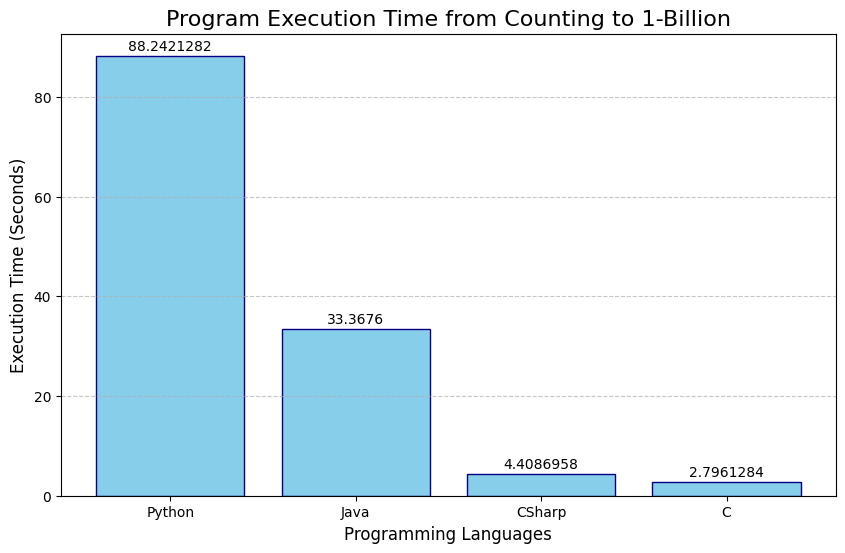
\includegraphics[width=0.8\textwidth]{../sync_records/sync_exec_times.png}
    \captionsetup{font=tiny, justification=centering}
    \caption{Execution time comparison of different programming languages running synchronously when counting from 1 to 1-billion.}
    \label{fig:sync-exec-times}
\end{figure}

The synchronous execution results above benchmark the time it took to compute the same task in each of the language. We saw expected results within most of the languages, with python having an average run time of 88 seconds, Java at 33, C\# 4 and C at a little less than 3 seconds. There was not much to note in these results, other than Java operating surprisingly slow when not using the JIT compiler.

\begin{figure}[!htb]
    \centering
    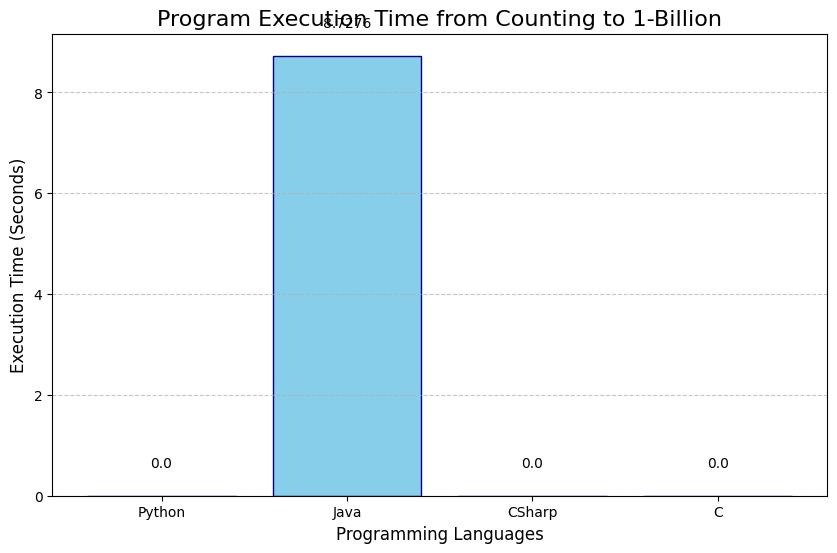
\includegraphics[width=0.8\textwidth]{../async_records/async_exec_times.png}
    \captionsetup{font=tiny, justification=centering}
    \caption{Execution time comparison of different programming languages running asynchronously with multi-threading when counting from 1 to 1-billion.}
    \label{fig:async-exec-times}
\end{figure}

The asynchronous execution results reveal a greater deal about the efficiency of the different programming languages however, as there was a big shift. Python was able to achieve a time of 43 seconds on average which amounts to a little more than twice the performance increase. Java was able to achieve an astounding 8.7 seconds, a little less than 4 times the performance increase. C\# was able to achieve an average time of 1.44 seconds, surprassing the performance of C, which was able to achieve an average time of 3.66 seconds, a significant reduction in performance.

When looking at these numbers for C, the first thought is that something must have gone wrong with the multi-core scheduling, as it got slower when attempting to run on multiple threads, but the System Monitor confirms that all four cores were actually being fully utilized, so then what could the reason be for this?

By now we have an idea about how threading is implemented in the various languages, and the thing that stands out the most is that C\# and Java both see the same performance increases when multi-threading. This is likely due to both languages having the same approach to threading as well as mapping onto kernel-level threads. Java utilizes the a Wrapper to wrest control of kernel threads, whilst C\# uses something more ambiguous within the .NET scheduler, but the end result is the same. This means that both languages are able to utilize almost the full potential of all the cores available in the system, and therefore we can expect significant performance increases when multi-threading in these specifically. 



\section{Discussion}

Include thoughts about other programming languages.

\section{Conclusion}

Add content if applicable.

\clearpage
\section{References}
\printbibliography
% Ensure Biber is run to resolve undefined references

\clearpage
\appendix

\section{Asynchronous Run-time Snippets}

\subsection{C Code Execution Times} 

\begin{figure}[htbp]
    \centering
    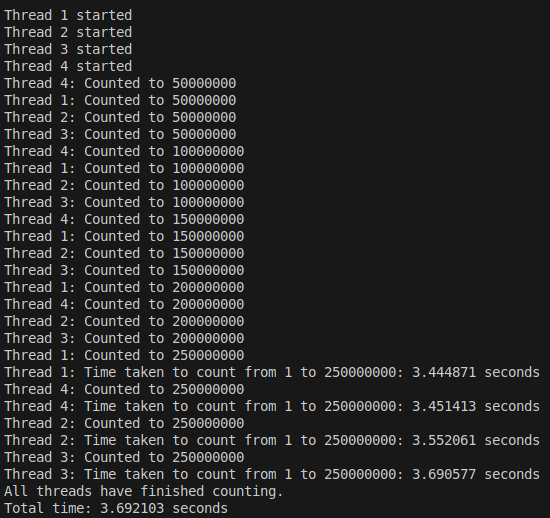
\includegraphics[width=0.8\textwidth]{../async_records/results_c/result_1.png}
    \caption{First run of asynchronous C code execution.}
    \label{fig:C-async-runtime-1}
\end{figure}

\begin{figure}[htbp]
    \centering
    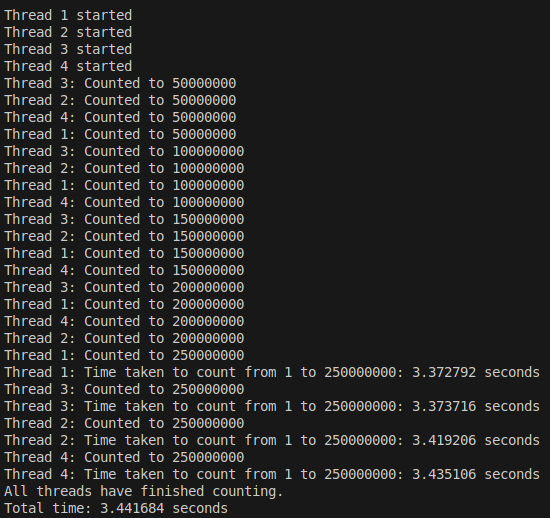
\includegraphics[width=0.8\textwidth]{../async_records/results_c/result_2.png}
    \caption{Second run of asynchronous C code execution.}
    \label{fig:C-async-runtime-2}
\end{figure}

\begin{figure}[htbp]
    \centering
    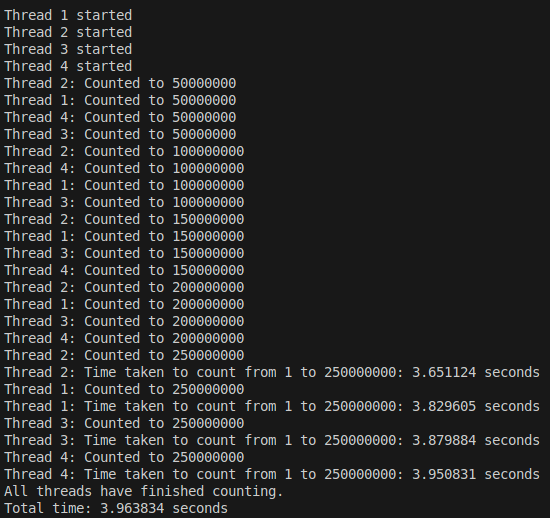
\includegraphics[width=0.8\textwidth]{../async_records/results_c/result_3.png}
    \caption{Third run of asynchronous C code execution.}
    \label{fig:C-async-runtime-3}
\end{figure}

\begin{figure}[htbp]
    \centering
    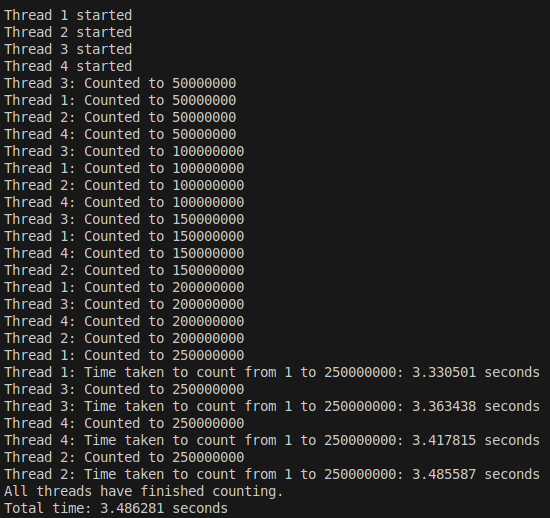
\includegraphics[width=0.8\textwidth]{../async_records/results_c/result_4.png}
    \caption{Fourth run of asynchronous C code execution.}
    \label{fig:C-async-runtime-4}
\end{figure}

\begin{figure}[htbp]
    \centering
    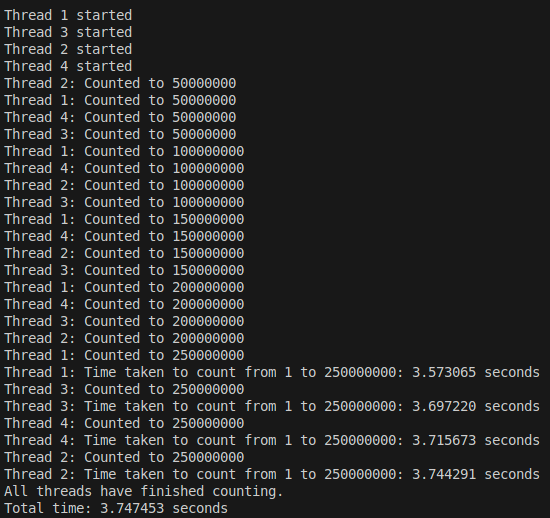
\includegraphics[width=0.8\textwidth]{../async_records/results_c/result_5.png}
    \caption{Fifth run of asynchronous C code execution.}
    \label{fig:C-async-runtime-5}
\end{figure}

\clearpage
\subsection{C-Sharp Code Execution Times} 

\begin{figure}[htbp]
    \centering
    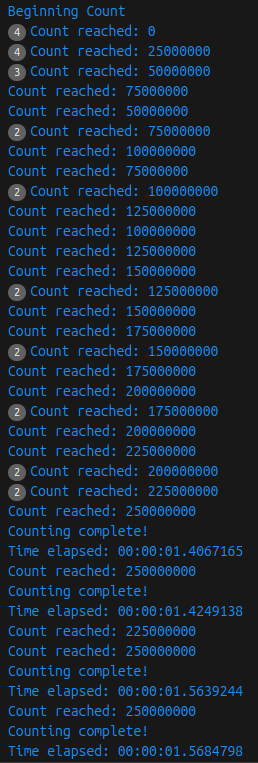
\includegraphics[width=0.8\textwidth]{../async_records/results_cs/result_1.png}
    \caption{First run of asynchronous C-Sharp code execution.}
    \label{fig:C-Sharp-async-runtime-1}
\end{figure}

\begin{figure}[htbp]
    \centering
    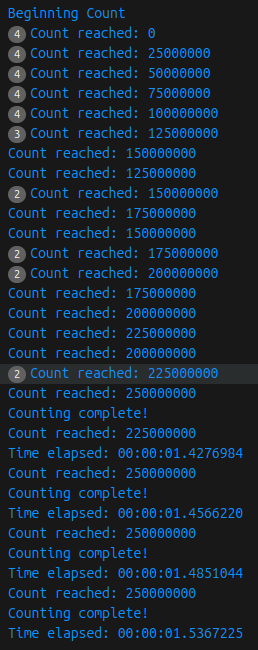
\includegraphics[width=0.8\textwidth]{../async_records/results_cs/result_2.png}
    \caption{Second run of asynchronous C-Sharp code execution.}
    \label{fig:C-Sharp-async-runtime-2}
\end{figure}

\begin{figure}[htbp]
    \centering
    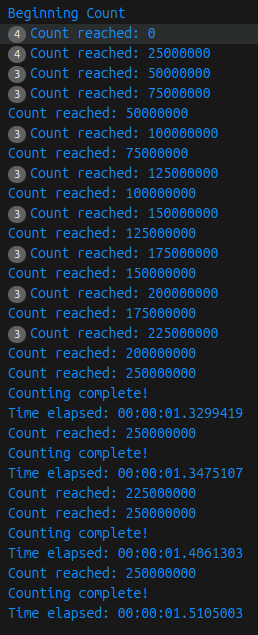
\includegraphics[width=0.8\textwidth]{../async_records/results_cs/result_3.png}
    \caption{Third run of asynchronous C-Sharp code execution.}
    \label{fig:C-Sharp-async-runtime-3}
\end{figure}

\begin{figure}[htbp]
    \centering
    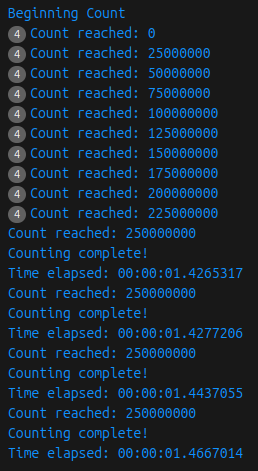
\includegraphics[width=0.8\textwidth]{../async_records/results_cs/result_4.png}
    \caption{Fourth run of asynchronous C-Sharp code execution.}
    \label{fig:C-Sharp-async-runtime-4}
\end{figure}

\begin{figure}[htbp]
    \centering
    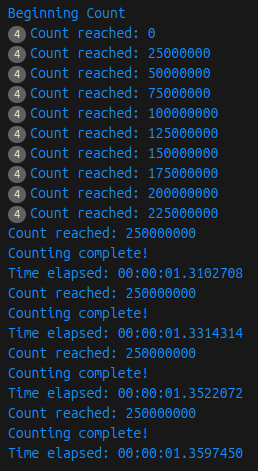
\includegraphics[width=0.8\textwidth]{../async_records/results_cs/result_5.png}
    \caption{Fifth run of asynchronous C-Sharp code execution.}
    \label{fig:C-Sharp-async-runtime-5}
\end{figure}

\clearpage
\subsection{Java Execution Times} 

\begin{figure}[htbp]
    \centering
    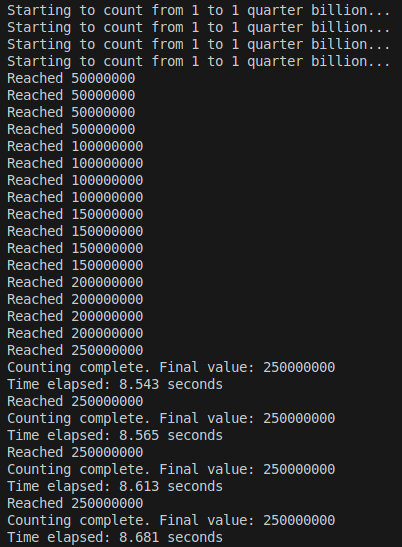
\includegraphics[width=0.8\textwidth]{../async_records/results_java/result_1.png}
    \caption{First run of asynchronous Java code execution.}
    \label{fig:Java-async-runtime-1}
\end{figure}

\begin{figure}[htbp]
    \centering
    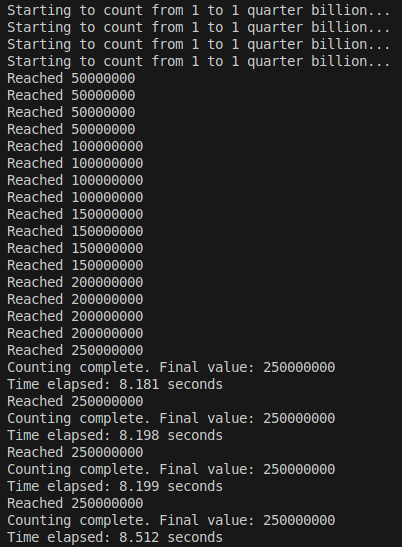
\includegraphics[width=0.8\textwidth]{../async_records/results_java/result_2.png}
    \caption{Second run of asynchronous Java code execution.}
    \label{fig:Java-async-runtime-2}
\end{figure}

\begin{figure}[htbp]
    \centering
    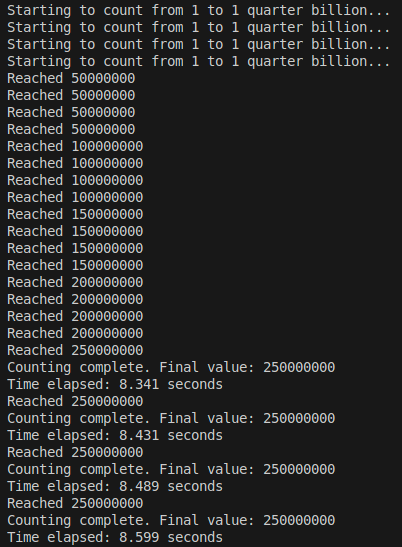
\includegraphics[width=0.8\textwidth]{../async_records/results_java/result_3.png}
    \caption{Third run of asynchronous Java code execution.}
    \label{fig:Java-async-runtime-3}
\end{figure}

\begin{figure}[htbp]
    \centering
    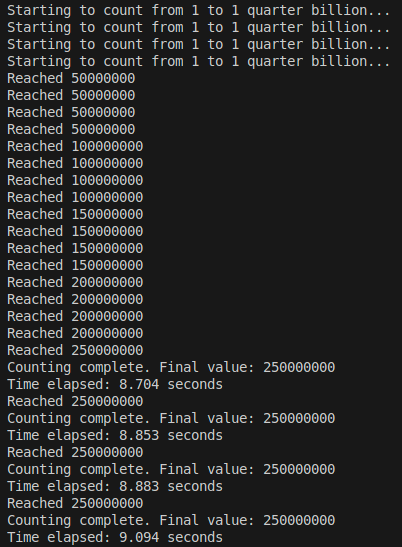
\includegraphics[width=0.8\textwidth]{../async_records/results_java/result_4.png}
    \caption{Fourth run of asynchronous Java code execution.}
    \label{fig:Java-async-runtime-4}
\end{figure}

\begin{figure}[htbp]
    \centering
    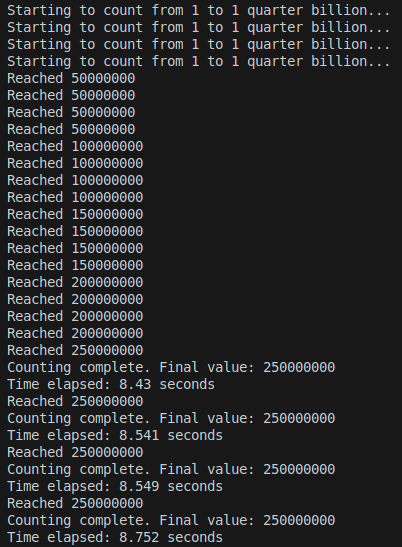
\includegraphics[width=0.8\textwidth]{../async_records/results_java/result_5.png}
    \caption{Fifth run of asynchronous Java code execution.}
    \label{fig:Java-async-runtime-5}
\end{figure}

\clearpage
\subsection{Python Execution Times} 

\begin{figure}[htbp]
    \centering
    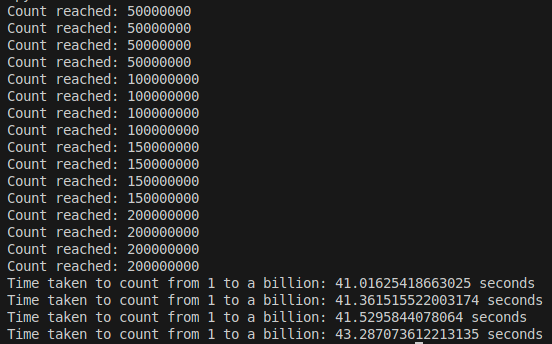
\includegraphics[width=0.8\textwidth]{../async_records/results_python/result_1.png}
    \caption{First run of asynchronous Python code execution.}
    \label{fig:Python-async-runtime-1}
\end{figure}

\begin{figure}[htbp]
    \centering
    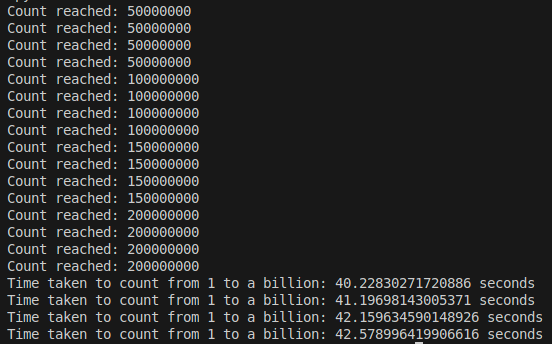
\includegraphics[width=0.8\textwidth]{../async_records/results_python/result_2.png}
    \caption{Second run of asynchronous Python code execution.}
    \label{fig:Python-async-runtime-2}
\end{figure}

\begin{figure}[htbp]
    \centering
    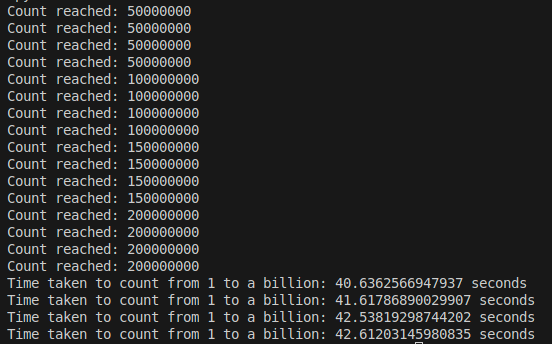
\includegraphics[width=0.8\textwidth]{../async_records/results_python/result_3.png}
    \caption{Third run of asynchronous Python code execution.}
    \label{fig:Python-async-runtime-3}
\end{figure}

\begin{figure}[htbp]
    \centering
    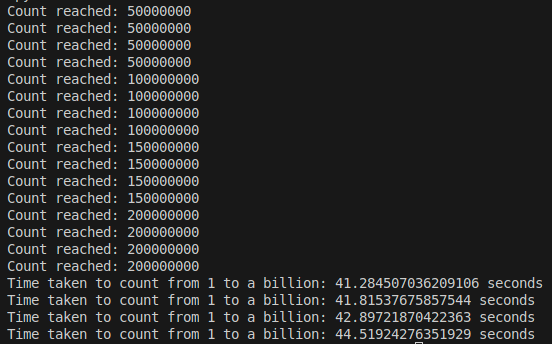
\includegraphics[width=0.8\textwidth]{../async_records/results_python/result_4.png}
    \caption{Fourth run of asynchronous Python code execution.}
    \label{fig:Python-async-runtime-4}
\end{figure}

\begin{figure}[htbp]
    \centering
    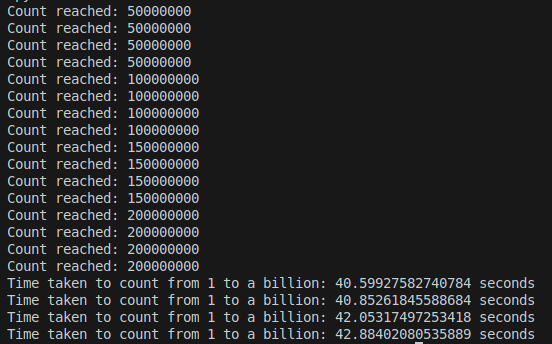
\includegraphics[width=0.8\textwidth]{../async_records/results_python/result_5.png}
    \caption{Fifth run of asynchronous Python code execution.}
    \label{fig:Python-async-runtime-5}
\end{figure}

\clearpage
\section{Synchronous Run-time Snippets}

\subsection{C Code Execution Times} 

\begin{figure}[htbp]
    \centering
    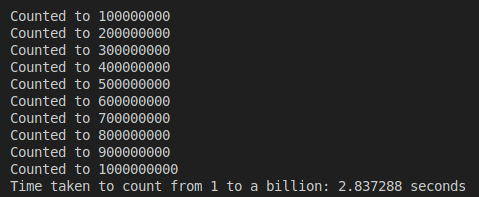
\includegraphics[width=0.8\textwidth]{../sync_records/results_c/result_1.png}
    \caption{First run of synchronous C code execution.}
    \label{fig:C-runtime-1}
\end{figure}

\begin{figure}[htbp]
    \centering
    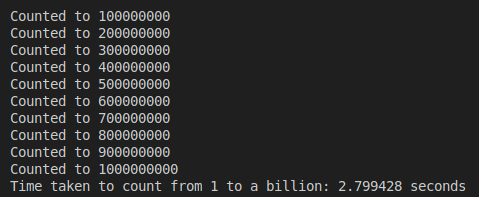
\includegraphics[width=0.8\textwidth]{../sync_records/results_c/result_2.png}
    \caption{Second run of synchronous C code execution.}
    \label{fig:C-runtime-2}
\end{figure}

\begin{figure}[htbp]
    \centering
    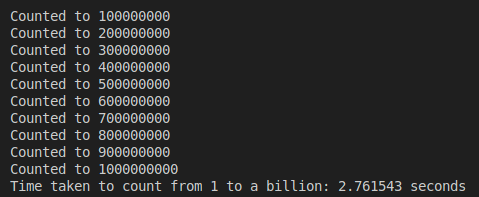
\includegraphics[width=0.8\textwidth]{../sync_records/results_c/result_3.png}
    \caption{Third run of synchronous C code execution.}
    \label{fig:C-runtime-3}
\end{figure}

\begin{figure}[htbp]
    \centering
    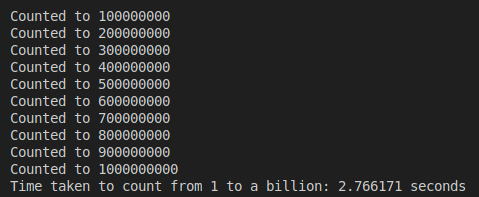
\includegraphics[width=0.8\textwidth]{../sync_records/results_c/result_4.png}
    \caption{Fourth run of synchronous C code execution.}
    \label{fig:C-runtime-4}
\end{figure}

\begin{figure}[htbp]
    \centering
    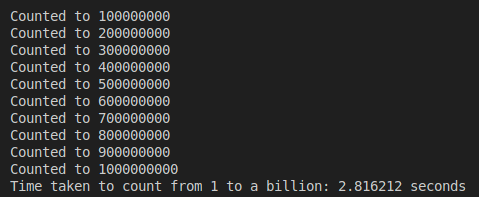
\includegraphics[width=0.8\textwidth]{../sync_records/results_c/result_5.png}
    \caption{Fifth run of synchronous C code execution.}
    \label{fig:C-runtime-5}
\end{figure}

\clearpage
\subsection{C-Sharp Code Execution Times} 

\begin{figure}[htbp]
    \centering
    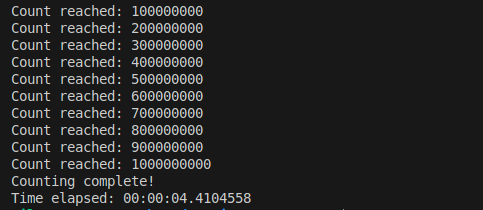
\includegraphics[width=0.8\textwidth]{../sync_records/results_cs/result_1.png}
    \caption{First run of synchronous C-Sharp code execution.}
    \label{fig:C-Sharp-runtime-1}
\end{figure}

\begin{figure}[htbp]
    \centering
    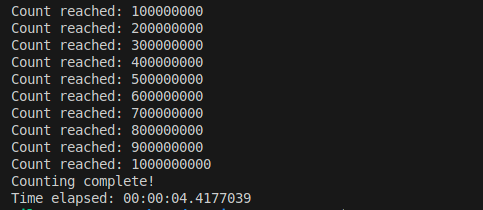
\includegraphics[width=0.8\textwidth]{../sync_records/results_cs/result_2.png}
    \caption{Second run of synchronous C-Sharp code execution.}
    \label{fig:C-Sharp-runtime-2}
\end{figure}

\begin{figure}[htbp]
    \centering
    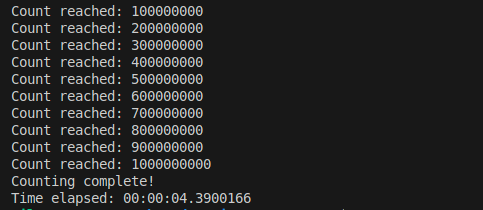
\includegraphics[width=0.8\textwidth]{../sync_records/results_cs/result_3.png}
    \caption{Third run of synchronous C-Sharp code execution.}
    \label{fig:C-Sharp-runtime-3}
\end{figure}

\begin{figure}[htbp]
    \centering
    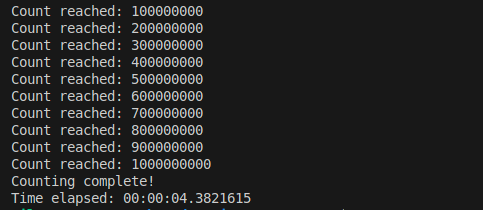
\includegraphics[width=0.8\textwidth]{../sync_records/results_cs/result_4.png}
    \caption{Fourth run of synchronous C-Sharp code execution.}
    \label{fig:C-Sharp-runtime-4}
\end{figure}

\begin{figure}[htbp]
    \centering
    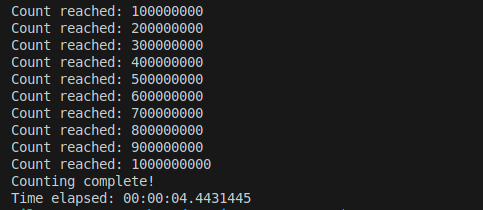
\includegraphics[width=0.8\textwidth]{../sync_records/results_cs/result_5.png}
    \caption{Fifth run of synchronous C-Sharp code execution.}
    \label{fig:C-Sharp-runtime-5}
\end{figure}

\clearpage
\subsection{Java Execution Times} 

\begin{figure}[htbp]
    \centering
    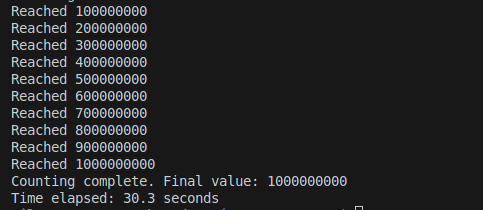
\includegraphics[width=0.8\textwidth]{../sync_records/results_java/result_1.png}
    \caption{First run of synchronous Java code execution.}
    \label{fig:Java-runtime-1}
\end{figure}

\begin{figure}[htbp]
    \centering
    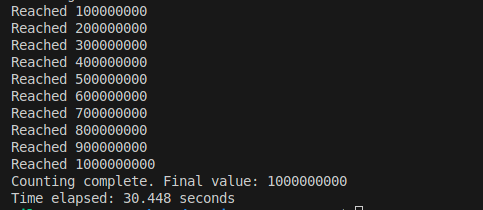
\includegraphics[width=0.8\textwidth]{../sync_records/results_java/result_2.png}
    \caption{Second run of synchronous Java code execution.}
    \label{fig:Java-runtime-2}
\end{figure}

\begin{figure}[htbp]
    \centering
    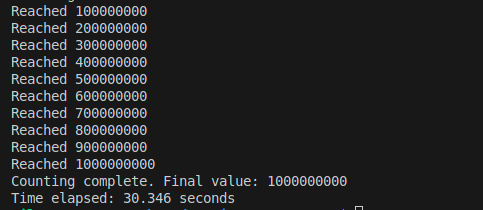
\includegraphics[width=0.8\textwidth]{../sync_records/results_java/result_3.png}
    \caption{Third run of synchronous Java code execution.}
    \label{fig:Java-runtime-3}
\end{figure}

\begin{figure}[htbp]
    \centering
    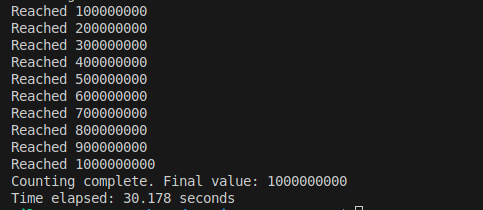
\includegraphics[width=0.8\textwidth]{../sync_records/results_java/result_4.png}
    \caption{Fourth run of synchronous Java code execution.}
    \label{fig:Java-runtime-4}
\end{figure}

\begin{figure}[htbp]
    \centering
    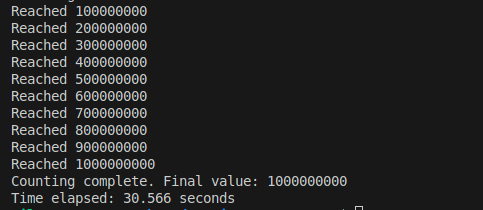
\includegraphics[width=0.8\textwidth]{../sync_records/results_java/result_5.png}
    \caption{Fifth run of synchronous Java code execution.}
    \label{fig:Java-runtime-5}
\end{figure}

\clearpage
\subsection{Python Execution Times} 

\begin{figure}[htbp]
    \centering
    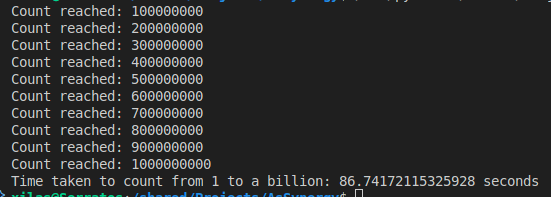
\includegraphics[width=0.8\textwidth]{../sync_records/results_python/result_1.png}
    \caption{First run of synchronous Python code execution.}
    \label{fig:Python-runtime-1}
\end{figure}

\begin{figure}[htbp]
    \centering
    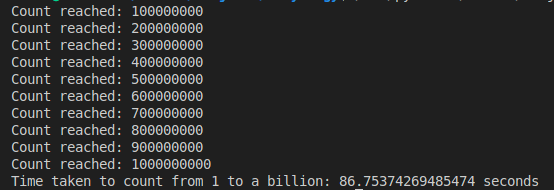
\includegraphics[width=0.8\textwidth]{../sync_records/results_python/result_2.png}
    \caption{Second run of synchronous Python code execution.}
    \label{fig:Python-runtime-2}
\end{figure}

\begin{figure}[htbp]
    \centering
    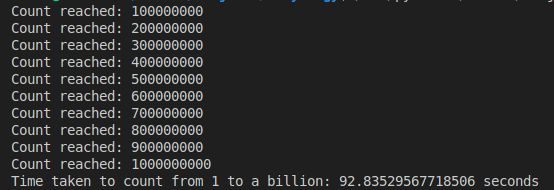
\includegraphics[width=0.8\textwidth]{../sync_records/results_python/result_3.png}
    \caption{Third run of synchronous Python code execution.}
    \label{fig:Python-runtime-3}
\end{figure}

\begin{figure}[htbp]
    \centering
    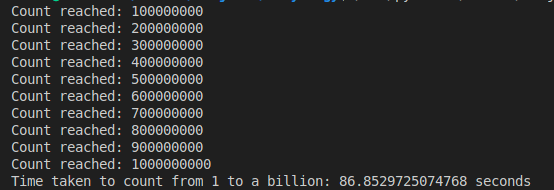
\includegraphics[width=0.8\textwidth]{../sync_records/results_python/result_4.png}
    \caption{Fourth run of synchronous Python code execution.}
    \label{fig:Python-runtime-4}
\end{figure}

\begin{figure}[htbp]
    \centering
    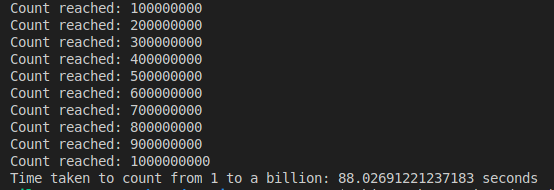
\includegraphics[width=0.8\textwidth]{../sync_records/results_python/result_5.png}
    \caption{Fifth run of synchronous Python code execution.}
    \label{fig:Python-runtime-5}
\end{figure}

\end{document}